%!TEX root = popl2018.tex


\section{Decision procedure for $\strline[\replaceall]$: The single-letter case} \label{sec:replaceallsl}





%%%%%%%%%%%%%%%%%%%%%%%%%%%%%%%%%
%%%%%%%%%%%%%%%%%%%%%%%%%%%%%%%%%
\hide{
\subsection{Encode concatenation by replaceall}

We will transform a given constraint $\varphi$ into a constraint $\varphi'$ which is concatenation free. As the first step, we extend the original alphabet with two fresh letters $a,b$. 

For each $x=yz$, we introduce a new variable $x'$ and replace $x=yz$ by two new constraints 
$x'=\replaceall(ab, a, x)$ and $x=\replaceall(x', b, z)$. 

\begin{proposition}
	$\varphi$ and $\varphi'$ are equisatisfiable. 	
\end{proposition}
}
%%%%%%%%%%%%%%%%%%%%%%%%%%%%%%%%%
%%%%%%%%%%%%%%%%%%%%%%%%%%%%%%%%%


%\subsection{The single-letter case}

In this section, we consider the single-letter case, that is, for the $\strline[\replaceall]$ formula $C = \varphi \wedge \psi$, every term of the form $\replaceall(z, e, z')$ in $\varphi$ satisfies that $e=a$ for $a \in \Sigma$.

%We first assume that the regular constraint $\psi = \bigwedge \limits_{x \in \vars(\varphi)} x \in e_x$, that is, there is exactly one atomic regular constraint for each variable.

%We first explain the basic idea of the decision procedure.

Let us start with the simple case that 
\[C \equiv x = \replaceall(y, a, z) \wedge x \in e_1 \wedge y \in e_2 \wedge z \in e_3,\]  
where, for $i =1, 2, 3$, suppose  $\cA_i = (Q_i, \delta_i, q_{0,i}, F_i)$ 
%\cA_y = (Q_y, \delta_y, q_{0, y}, F_y), \cA_z = (Q_z, \delta_z, q_{0, z}, F_z)$ 
is the NFA corresponding to $e_i$. 

$C$ is satisfiable if and only if $x, y, z$ can be assigned with strings $u, v, w$ so that: (1) $u$ is obtained from $v$ by replacing all the occurrences of $a$ in $v$ with $w$, and (2) $u, v, w$ are accepted by $\cA_1, \cA_2, \cA_3$ respectively. As $u$ is accepted by $\cA_1$,  there must be an accepting run of $\cA_1$ on $u$. Let $v = v_1 a v_2 a \cdots a v_k$ such that for each $i \in [k]$, $v_i \in (\Sigma \setminus \{a\})^*$. Then $u = v_1 w v_2 w \cdots w v_k$ and there are states $q_1, q'_1, \cdots, q_{k-1}, q'_{k-1}, q_k$  such that 
%
$$
q_{0,1} \xrightarrow[\cA_1]{v_1} q_1 \xrightarrow[\cA_1]{w} q'_1 \xrightarrow[\cA_1]{v_2} q_2 \xrightarrow[\cA_1]{w} q'_2 \cdots q_{k-1} \xrightarrow[\cA_1]{w} q'_{k-1} \xrightarrow[\cA_1]{v_k} q_k
$$
%
 and $q_k \in F_{1}$. Let $T_z$ denote $\left\{(q_i, q'_i) \mid i \in [k-1] \right\}$. Then $w \in \Ll(\cA_3)\ \cap\ \bigcap \limits_{(q, q') \in T_z} \Ll(\cA_1(q, q'))$. In addition, let  $\cB_{\cA_1,a,T_z}$ be the NFA obtained from $\cA_1$ by removing all the $a$-transitions first and then adding the $a$-transitions $(q, a, q')$ for $(q, q') \in T_z$. Then 
 %
$$
q_{0,1} \xrightarrow[\cB_{\cA_1,a,T_z}]{v_1} q_1 \xrightarrow[\cB_{\cA_1,a,T_z}]{a} q'_1 \xrightarrow[\cB_{\cA_1,a,T_z}]{v_2} q_2 \xrightarrow[\cB_{\cA_1,a,T_z}]{a} q'_2 \cdots q_{k-1} \xrightarrow[\cB_{\cA_1,a,T_z}]{a} q'_{k-1} \xrightarrow[\cB_{\cA_1,a,T_z}]{v_k} q_k.
$$
%
Therefore, 
$v \in \Ll(\cA_2) \cap \Ll(\cB_{\cA_1,a,T_z})$. We deduce that there is $T_z \subseteq Q_1 \times Q_1$ such that $\Ll(\cA_3)\ \cap\ \bigcap \limits_{(q, q') \in T_z} \Ll(\cA_1(q, q')) \neq \emptyset$ and $ \Ll(\cA_2) \cap \Ll(\cB_{\cA_1,a,T_z}) \neq \emptyset$. In addition, it is not hard to see that this condition is also sufficient for the satisfiability of $C$. \zhilin{to be more specific}

\begin{proposition}\label{prop-sat-sl-case}
Let $C \equiv x = \replaceall(y, a, z) \wedge x \in e_1 \wedge y \in e_2 \wedge z \in e_3$. Then $C$ is satisfiable iff there is a set $T_{z} \subseteq Q_1 \times Q_1$ such that $\Ll(\cA_3)\ \cap\ \bigcap \limits_{(q, q') \in T_z} \Ll(\cA_1(q, q')) \neq \emptyset$ and $ \Ll(\cA_2) \cap \Ll(\cB_{\cA_1,a,T_z}) \neq \emptyset$.
\end{proposition}

From Proposition~\ref{prop-sat-sl-case}, we can decide the satisfiability of $C$ in polynomial space as follows: 
\begin{description}
\item[Step I.] Guess a set $T_{z} \subseteq Q_1 \times Q_1$. 
%
\item[Step II.] Guess an accepting run of the product automaton of $\cA_3$ and $\cA_1(q, q')$ for $(q,q') \in T_{z}$. 
%
\item[Step III.] Guess an accepting run of the product automaton of $\cA_2$ and $\cB_{\cA_1, a,  T_{z}}$. 
\end{description}
During Step II and III, it is sufficient to record $T_z$ and a state of the product automaton, which occupies only a polynomial space.

The above decision procedure can be easily generalised to the case that there are multiple atomic regular constraints for $x$. For instance, let $x \in e_{1,1} \wedge x \in e_{1,2}$ and for $j = 1, 2$, $\cA_{1,j} = (Q_{1,j}, \delta_{1, j}, q_{0,1, j}, F_{1,j})$ be 
the NFA corresponding to $e_{1,j}$. Then in Step I, two sets $T_{1,z} \subseteq Q_{1,1} \times Q_{1,1}$ and $T_{2,z} \subseteq Q_{1,2} \times Q_{1,2}$ are guessed, moreover, Step II and III are adjusted accordingly.

\begin{example}
Let $C \equiv x= \replaceall(y, 0, z) \wedge x \in e_1 \wedge y \in e_2 \wedge z \in e_3$, where $e_1=(0+1)^* (00(0+1)^* + 11(0+1)^*)$,  $e_2= (01)^*$,  and $e_3 = (10)^*$. The NFA $\cA_{1}, \cA_{2}, \cA_{3}$ corresponding to $e_1, e_2, e_3$ respectively are illustrated in Figure~\ref{fig-sl-exmp}. Let $T_z = \{(q_0, q_0), (q_1, q_2)\}$.  Then 
$$
\begin{array}{l c l}
 \Ll(\cA_3)\ \cap\ \bigcap \limits_{(q, q') \in T_z} \Ll(\cA_1(q, q'))  & = & \Ll(\cA_3)\ \cap \Ll(\cA_1(q_0, q_0)) \cap \Ll(\cA_1(q_1,q_2)) \\
& = & \Ll((10)^*) \cap \Ll((0+1)^*) \cap \Ll(1(0+1)^*) \\
& \neq & \emptyset.
\end{array}
$$
In addition, $\cB_{\cA_1, 0, T_z}$ (also illustrated in Figure~\ref{fig-sl-exmp}) is obtained from $\cA_1$ by removing all the $0$-transitions, then adding the transitions $(q_0, 0, q_0)$ and $(q_1, 0, q_2)$. Then
$$
 \Ll(\cA_2) \cap \Ll(\cB_{\cA_1,0,T_z})   =  (01)^* \cap (0+1)^* 10 1^* \neq \emptyset.
$$
Therefore, we can choose $z$ to be a string from $\Ll(\cA_3) \cap \ \bigcap \limits_{(q, q') \in T_z} \Ll(\cA_1(q, q'))=\Ll((10)^*) \cap \Ll((0+1)^*) \cap \Ll(1(0+1)^*)$, say $10$, and $y$ to be a string from $ \Ll(\cA_2) \cap \Ll(\cB_{\cA_1,0,T_z})   =  (01)^* \cap (0+1)^* 10 1^*$, say $0101$,  then $x$ gets the value $\replaceall(0101, 0, 10)=101101$, which is in $\Ll(\cA_1)$. Therefore, $C$ is satisfiable.
\begin{figure}[htbp]
\begin{center}
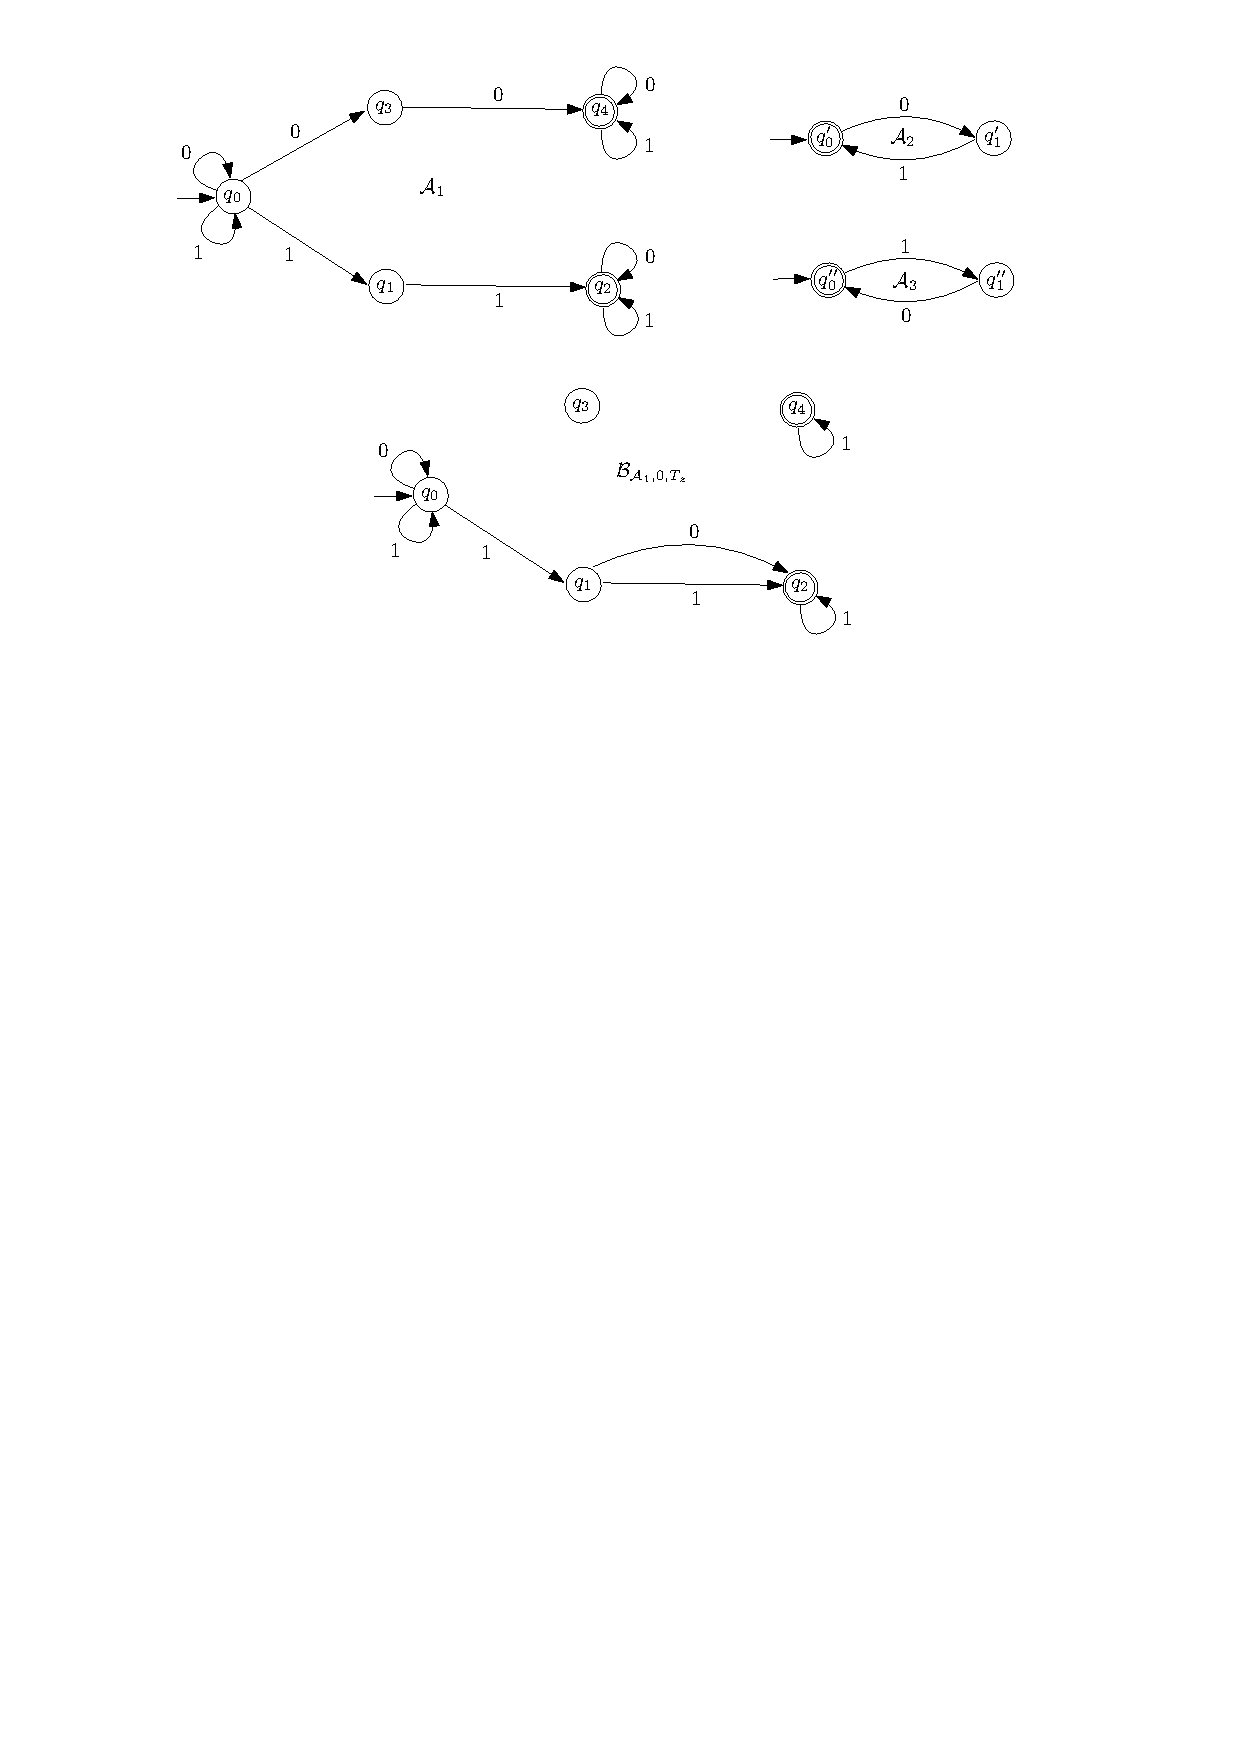
\includegraphics[scale=0.8]{single-letter-example.pdf}
\end{center}
\caption{An example for single-letter case}\label{fig-sl-exmp}
\end{figure}
\end{example}

Let us now consider the general case that $C$ contains multiple occurrences of $\replaceall(\cdots)$ terms. 
Then the satisfiability of $C$ is decided by the following two-step procedure.

\smallskip

\noindent{\bf Step I.} We utilise the dependency graph $C$ and compute nondeterministically a collection of atomic regular constraints $\cE(x)$ for each variable $x$, in a top-down manner. 

%During the computation, for each variable $x$, the collection of atomic regular constraints 
Notice that $\cE(x)$ is represented succinctly as a set of pairs $(\cT, \cP)$, where $\cT=(Q, \delta)$ is a transition graph and $\cP \subseteq Q \times Q$. The intention of $(\cT, \cP)$ is to represent succinctly the collection of the atomic regular constraints $(Q, \delta, q, \{q'\})$, where $q$ is the initial state and $\{q'\}$ is the set of final states, for $(q,q') \in \cP$. \tl{you want to say that all regular constraints $\cE(x)$ share the same "underlying" graph, but differ in the initial and final states.}

\tl{I rephrased a bit-- the original was commented below. Check whether this is what you mean}

Initially, let $G_0:= G_C$.  In addition, for each variable $x$ with the conjunct $x \in e$ in $\psi$, let $\cA=(Q, \delta, q_0, F)$ be the NFA corresponding to $e$. We nondeterministically choose $q \in F$ and let $\cE_0(x):=  \{((Q, \delta), \{(q_0, q)\})\}$.


%In addition, for each variable $x$, compute $\cE_0(x)$ as follows: Initially, let $\cE_0(x) := \emptyset$.
%For each conjunct $x \in e$ in $\psi$, let $\cA=(Q, \delta, q_0, F)$ be the NFA corresponding to $e$, then nondeterministically choose $q \in F$ and let $\cE_0(x):= \cE_0(x) \cup \{((Q, \delta), \{(q_0, q)\})\}$.
% 

Let $i: = 0$ and repeat the following procedure until $G_i$ becomes an empty graph, i.e. a graph without edges. 
\begin{enumerate}
\item Select a vertex $x$ of $G_i$ such that $x$ has no predecessors \tl{parent} and has two successors in $G_i$. Suppose $(x, (\rpleft, a), y)$ and $(x, (\rpright,a), z)$ are the two edges out of $x$ in $G_i$ and $\cE_i(x)=\{(\cT_1,\cP_1), \cdots, (\cT_k, \cP_k)\}$, where for each $j \in [k]$, $\cT_j = (Q_j, \delta_j)$. Then $\cE_{i+1}(z)$ and  $\cE_{i+1}(y)$ and $G_{i+1}$ are computed as follows:  
\begin{enumerate}
\item For each $j \in [k]$, guess a set $T_{j, z} \subseteq Q_j \times Q_j$.
%
\item If $y \neq z$, then let 
$$\cE_{i+1}(z):= \cE_{i}(z) \cup \left\{(\cT_j, T_{j,z}) \mid j \in [k] \right\}$$
and 
$$\cE_{i+1}(y): = \cE_{i}(y) \cup \left\{(\cT_{\cA_j, a, T_{j,z}}, \cP_j) \mid j \in [k] \right\},$$
where $\cT_{\cA_j, a, T_{j,z}}$ is the transition graph of $\cB_{\cA_j, a, T_{j,z}}$. 

Otherwise, let
$$\cE_{i+1}(z):= \cE_{i}(z) \cup \left\{(\cT_j, T_{j,z}) \mid j \in [k] \right\} \cup \left\{(\cT_{\cA_j, a, T_{j,z}}, \cP_j) \mid j \in [k] \right\}.$$
In addition, for each vertex $x'$ distinct from $y, z$, let $\cE_{i+1}(x') := \cE_i(x')$.
%
\item Let $G_{i+1}:= G_i \setminus \{(x, (\rpleft, a), y), (x, (\rpright,a), z)\}$.
\end{enumerate}
%
\item Let $i: = i+1$.
\end{enumerate}

For each variable $x$, let $\cE(x)$ denote the set $\cE_i(x)$ after exiting the above loop. 

\smallskip

\noindent {\bf Step II.} 
For each source variable $x$, guess an accepting run of the product automaton of all the NFA in $\cE(x)$. 

\smallskip

%Note that in the first sight, the cardinalities of the sets $\cE(x)$ seem exponential w.r.t. the size of $C$ in the worst case and the nondeterministic algorithm may take exponential space. 
%By a refined analysis, we can see that the cardinalities of the sets $\cE(x)$ are in fact polynomial. 

To show that the aforementioned nondeterministic decision procedure works in exponential space, it is sufficient to show that the cardinalities of the sets $\cE(x)$ are exponential w.r.t. the size of $C$. 

\begin{proposition}
The cardinalities of $\cE(x)$ for the variables $x$ in $G_C$ are at most exponential  in the size of $C$ and become polynomial for $\strline_{\sf ss}[\replaceall]$ formuale.
\end{proposition}

\begin{proof}
%The transition graphs $\cT=(Q, \delta)$ and $\cT'=(Q', \delta')$ are said to be \emph{isomorphic} if there is a bijection $\pi: Q \rightarrow Q'$ such that for each $q, q' \in Q$ and $a \in \Sigma$, $(q, a, q') \in \delta$ iff $(\pi(q), a, \pi(q')) \in \delta'$.
%
Let $K$ denote the maximum cardinality of $\cE_0(x)$ for vertices $x$ in $G_C$. 
%In addition, for each node $x$ in $G_C$, let $\#^{\sf anc}$ 
%In addition, let $M$ denote the maximum size (number of states) of the NFA in $\cE_0(x)$ for nodes $x$ in $G_C$. 
For each $i$ and each vertex $x$ in $G_C$, let  $\#^{\sf anc}_i(x)$ denote the number of ancestors of $x$ in $G_i$.
%, in addition, let ${\sf Idx}^{\sf arb}_i(x)$ denote the maximum number of join vertices in a path starting from $x$ in $G_i$.

%the number of edges of $G_0 \setminus G_i$ (i.e. the subgraph of $G_0$ comprising all the edges not in $G_i$) that are co-reachable from $x$ in  $G_0 \setminus G_i$. 

% and $\#_{\sf lft}(x)$ denote the number of $\rpleft$-edges that are co-reachable from $x$ in $G_C$.

%Then the proposition follows from the following claim, since for each node $x$, $|\cE(x)| \le |\cG(\cE(x))|M^2$.

We first prove the following claim.

\smallskip

\noindent {\bf Claim}. For each $i$ and each vertex $x$ in $G_C$, 
$|\cE_i(x)| \le 3^i K$. In addition, if $C \in \strline_{\sf ss}[\replaceall]$, then for each non-source variable $x$ in $G_C$, $|\cE_i(x)| \le (\#^{\sf anc}_0(x)-\#^{\sf anc}_i(x)+1) K$.
%In addition, if $G_C$ is a tree, then $|\cE_i(x)| \le (\#^{\sf anc}_0(x)-\#^{\sf anc}_i(x)+1) K$.

\smallskip

We prove the claim by an induction on $i$.

\smallskip


\noindent {\it Induction base}: $i=0$. Evidently $|\cE_0(x)| \le K = 3^0 K$. Moreover, if $C \in \strline_{\sf ss}[\replaceall]$, then for each non-source variable $x$, $|\cE_0(x)| \le K = (\#^{\sf anc}_0(x)-\#^{\sf anc}_0(x)+1) K$.
% = (\#^{\sf anc}_0(x)-\#^{\sf anc}_0(x)+1) K$.

\smallskip

\noindent {\it Induction step}: 
Suppose $i > 0$.

Let $x$ be the vertex without predecessors and with successors in $G_{i-1}$ that is used to construct $G_{i}$. In addition, let $(x, (\rpleft, a), y)$ and $(x, (\rpright, a), z)$ be the two edges out of $x$ in $G_{i-1}$.

Let us first assume $y \neq z$.
Then $|\cE_{i}(z)| \le |\cE_{i-1}(z)| + |\cE_{i-1}(x)|$ and $|\cE_{i}(y)| \le |\cE_{i-1}(y)| + |\cE_{i-1}(x)|$.  By the induction hypothesis, $|\cE_{i-1}(x)| \le  3^{i-1} K$, $|\cE_{i-1}(y)| \le 3^{i-1} K$, and $|\cE_{i-1}(z)| \le 3^{i-1} K$. Therefore, $|\cE_{i}(z)|  \le |\cE_{i-1}(z)| + |\cE_{i-1}(x)| \le 3^{i-1} K + 3^{i-1} K \le 3^i K$. Similarly, $|\cE_{i}(y)| \le 3^i K$.

Next, we assume $y = z$. Then $|\cE_{i}(z)| \le |\cE_{i-1}(z)| + |\cE_{i-1}(x)| + |\cE_{i-1}(x)| \le 3* 3^{i-1} K = 3^i K$. 

Let us assume that $C \in \strline_{\sf ss}[\replaceall]$, moreover, either $y$ or $z$ is not a source variable. Then $y \neq z$. Because otherwise, the in-degree of $y=z$ in $G_C$ is more than one, from the fact that $G_C$ is source-sharing, we deduce that $y=z$ has to be a source variable, a contradiction. Let us first assume that $z$ is not a source variable. Then the in-degree of $z$ is one, that is, the edge from $x$ to $z$ is the only incoming edge of $z$ in $G_C$. From this, we deduce that  $\cE_{i-1}(z) = \cE_0(z)$. Therefore, $|\cE_{i}(z)| \le |\cE_{i-1}(z)| + |\cE_{i-1}(x)| \le K + |\cE_{i-1}(x)|$. By the induction hypothesis, $|\cE_{i-1}(x)| \le (\#^{\sf anc}_{0}(x) - \#^{\sf anc}_{i-1}(x)+1)K$. We deduce that $|\cE_{i}(z)| \le K+ (\#^{\sf anc}_{0}(x) - \#^{\sf anc}_{i-1}(x)+1)K$. Moreover, since $\#^{\sf anc}_{0}(z) = \#^{\sf anc}_{0}(x)+1$ and $\#^{\sf anc}_{i-1}(x)=\#^{\sf anc}_{i}(x)= \#^{\sf anc}_{i}(z)=0$, we have $|\cE_{i}(z)| \le K+ (\#^{\sf anc}_{0}(z)-1 - \#^{\sf anc}_{i}(z)+1)K = (\#^{\sf anc}_{0}(z) - \#^{\sf anc}_{i}(z)+1)K$.
Similarly, if $y$ is not a source variable, we have $|\cE_{i}(y)| \le |\cE_{i-1}(y)| + |\cE_{i-1}(x)| = |\cE_{0}(y)| + |\cE_{i-1}(x)| \le K+|\cE_{i-1}(x)| \le K+ (\#^{\sf anc}_{0}(x) - \#^{\sf anc}_{i-1}(x)+1)K \le K+ (\#^{\sf anc}_{0}(y)-1 - \#^{\sf anc}_{i}(y)+1)K = (\#^{\sf anc}_{0}(y) - \#^{\sf anc}_{i}(y)+1)K$.

The proof of the claim is complete.

Let $H$ be the maximum length of the paths in $G_C$. From the claim, we deduce that for each non-source variable $x$, $|\cE(x)| \le (H-1)K$. In addition, for each source variable $y$ in $G_C$, suppose that the in-degree of $y$ in $G_C$ is $m$, then $|\cE(y)| \le K + \sum \limits_{x: \mbox{ \small predecessor of } y} |\cE(x)| \le  K+m(H-1)K=(mH-m+1) K$.
%

Therefore, we conclude that if $C \in \strline_{\sf ss}[\replaceall]$, then the cardinalities of $\cE(x)$ become polynomial in the size of $C$. 
\end{proof}

%\begin{quote}
%\it Let $x$ be a node in the graph without predecessors and $x = \replaceall(y, a, z)$ be a conjunct of $\varphi$ and $\cA_1, \dots, \cA_m$ be a collection of regular constraints for $x$. Then remove the two edges out of $x$, guess $T_{i, z} \subseteq Q_i \times Q_i$ for $i \in [m]$, and add additional regular constraints to $y$ and $z$ as specified above. 
%\end{quote}

%For doing this, we need deal with the typical situation that $x = \replaceall(y, a, z)$  and the regular constraints for $x$ are specified by 

%We first introduce a concept of dependency graphs.


\begin{example}
\end{example}


%\begin{theorem}
%The satisfiability of $\pstrline[\replaceall]$ is in EXPSPACE and PSPACE-complete for formulae whose dependency graphs trees.
%\end{theorem}

\section{Decision procedure for $\strline[\replaceall]$: The constant-string case}

In this section, we consider the constant-string special case, that is, given an $\strline[\replaceall]$ formula $C = \varphi \wedge \psi$, it holds that every term of the form $\replaceall(z, e, z')$ in $\varphi$ satisfies that $e=u$ for $u \in \Sigma^+$.

Let us start with the simple case that $C \equiv x = \replaceall(y, u, z) \wedge \bigwedge \limits_{i \in [k]} x \in e_{i}$ such that $|u| \ge 2$.  In addition, for $i \in [k]$, suppose $\cA_i = (Q_i, \delta_i, q_{0, i}, F_i)$ 
%\cA_y = (Q_y, \delta_y, q_{0, y}, F_y), \cA_z = (Q_z, \delta_z, q_{0, z}, F_z)$ 
is the NFA corresponding to $e_i$. 
\begin{enumerate}
\item For each $i \in [k]$, we will guess a set $T_{i, z} \subseteq Q_i \times Q_i$, which intuitively means that in $\cA_i$, for each state pair $(q, q') \in T_{i, z}$, starting from $q$, after reading $z$, the state $q' $ can be reached. The functions $(T_{i, z})_{i \in [k]}$ induce regular constraints $\Ll(\cA_i(q,q'))$ on $z$, where $i \in [k]$ and $(q,q') \in T_{i, z}$.

\item For each $i \in [k]$, we construct an NFA $\cB_{\cA_i, u,  T_{i, z}}$, which specifies some additional regular constraint on $y$. Intuitively, a string $v$ is accepted by $\cB_{\cA_i, u,  T_{i, z}}$ iff either $v \not \in \Sigma^\ast u \Sigma^\ast$ and $v$ is accepted by $\cA_i$, or otherwise, let $v = v'_1 u v'_2 u \dots v'_{k-1} u v'_{k}$ such that $v'_i u' \not \in \Sigma^\ast u \Sigma^\ast$ for each $i \in [k-1]$ and each strict prefix $u'$ of $u$ and $v'_k \not \in \Sigma^\ast u \Sigma^\ast$, then $q_{i,0} \xrightarrow{v'_1} q_1 \xrightarrow{T_{i,z}} q'_1 \xrightarrow{v'_2} q_2 \xrightarrow{T_{i,z}} q'_2 \dots \xrightarrow{v'_{k-1}} q_{k-1} \xrightarrow{T_{i,z}} q'_{k-1} \xrightarrow{v'_k} q_k$ for states $q_1, q'_1, \dots, q_{k-1}, q'_{k-1}, q_k \in Q_i$ with $q_k \in F_{i,z}$. 
\end{enumerate}

In order to construct the NFA $\cB_{\cA_i, u,  T_{i, z}}$, we introduce concepts of window profiles and parsing automata defined below.

Let $u \in \Sigma^+$ and $k=|u| \ge 2$.


%If $u = \sigma$ for $\sigma \in \Sigma$, then $\cA_u=(Q_u, \delta_u, q_{0,u}, F_u)$, where $Q_u = \{(q_0, \bot), (q_0, \top) \}$, $\delta_u = \{(q_0, \bot) \xrightarrow{\sigma} (q_0, \top), (q_0, \bot) \xrightarrow{\Sigma \setminus \sigma} (q_0, \bot), (q_0, \top) \xrightarrow{ \sigma} (q_0, \top), (q_0, \top) \xrightarrow{\Sigma \setminus \sigma} (q_0, \bot)\}$, $q_{0,u} = (q_0, \bot)$, and $F_u = Q_u$.

%In the following, we assume that $|u| = k \ge 2$. Let $u = u_1 \dots u_k$, where each $u_i \in \Sigma$.

%We construct an NFA $\cA_u=(Q_u, \delta_u, q_{0,u}, F_u)$ which over a string $v$, parses $v \in \Sigma^\ast u \Sigma^\ast$ into $v_1 u v_2 u \dots v_l u v_{l+1}$ such that $v_j u_1 \dots u_{k-1} \not \in \Sigma^\ast u \Sigma^\ast$ for each $1 \le j \le l$, and $v_{l+1} \not \in \Sigma^\ast u \Sigma^\ast$. 
%Let $u = u_1\dots u_k$ such that $u_i \in \Sigma$ for each $i \in [k]$.  

\begin{definition}[$k$-window profiles w.r.t. $u$]
A $k$-\emph{window profile $\overrightarrow{W}$ w.r.t. $u$} is an element of $\{\bot,\top\}^{k-1}$. Intuitively, in the position $i$ of a string $v$, $\overrightarrow{W}$ is an abstraction of the substring $v[i-k+2] \dots v[i]$ such that for each $j \in [k-1]$, $\overrightarrow{W}(j) = \top$ iff $v[i-j+1] \dots v[i] = u[1] \dots u[j]$. Let $\wprof_{u, k}$ denote the set of $k$-window profiles w.r.t. $u$. 
%In particular, if $k = 1$, then $\wprof_{u, k} = \emptyset$. 
\end{definition}

%\zhilin{the following fact is noticed by Yan Chen.} 
\begin{proposition}
The number of $k$-window profiles w.r.t. $u$ is polynomial in the length of $u$. 
\end{proposition}
\begin{proof}
The arguments for this fact proceed as follows: For each profile $\overrightarrow{W}$, let $v$ be a string and $i$ be a position of $v$ such that for each $j \in [k-1]$, $\overrightarrow{W}(j) = \top$ iff $v[i-j+1] \dots v[i] = u[1] \dots u[j]$. Define ${\sf idx}_{\overrightarrow{W}}$ as the maximum index $j \in [k-1]$ such that $\overrightarrow{W}(j)=\top$. Then 
\begin{itemize}
	\item for each $j': j < j' < k$, $\overrightarrow{W}(j')=\bot$, 
	\item in addition, since $v[i-{\sf idx}_{\overrightarrow{W}}+1] \dots v[i] = u[1] \dots u[{\sf idx}_{\overrightarrow{W}}]$, the values of $\overrightarrow{W}(1),\dots, \overrightarrow{W}({\sf idx}_{\overrightarrow{W}})$ are completely determined by $u[1] \dots u[{\sf idx}_{\overrightarrow{W}}]$.
\end{itemize}
From the above arguments, we can  conclude that the number of $k$-window profile $\vec{W}$ w.r.t. $u$ is actually at most $k$.
\end{proof}

From $u$, we will construct a parsing automaton $\cA_u=(Q_u, \delta_u, q_{0,u}, F_u)$ which parses a string $v \in \Sigma^\ast u \Sigma^\ast$ into $v_1 u v_2 u \dots v_l u v_{l+1}$ such that $v_j u[1] \dots u[k-1] \not \in \Sigma^\ast u \Sigma^\ast$ for each $1 \le j \le l$, in addition, $v_{l+1} \not \in \Sigma^\ast u \Sigma^\ast$. 
The concept of $k$-window profiles w.r.t. $u$ are used to check that a substring of $v$ is \emph{not} in $\Sigma^\ast u \Sigma^\ast$.
Specifically, the NFA $\cA_u$ is constructed as follows.
\begin{itemize}
	\item  $Q_u =\{q_0\} \cup \{(\search, \overrightarrow{W}) \mid \overrightarrow{W} \in \wprof_{u, k}\} \cup \{(\verify, j, \overrightarrow{W}) \mid j \in [k-1], \overrightarrow{W} \in \wprof_{u,k}\}$, where $q_0$ is a distinguished state whose purpose will become clear later on,  $\search$ and $\verify$ are used to denote whether $\cA_u$ is in the ``search''-mode to search the next occurrence of $u$, or in the ``verify'' mode to verify that the current position is a part of an occurrence of $u$.
	%
	\item $q_{0,u}=q_0$.
	
	\item $\delta_{u}$ comprises the following transitions,
	%guesses over each position, one of the following holds, the substring comprising the next $k$-symbols (including the current one) is $u$ or not.
	\begin{itemize}
		\item $q_0 \xrightarrow{\sigma} (\search, \overrightarrow{W})$, where $\overrightarrow{W}(1)=\top$ iff $\sigma = u[1]$, and for each $i: 2 \le i \le k-1$, $\overrightarrow{W}(i) = \bot$,
		%
		\item for each state $(\search, \overrightarrow{W})$ and $\sigma \in \Sigma$ such that $\overrightarrow{W}(k-1) = \bot$ or $\sigma \neq u[k]$,
		\begin{itemize}
			\item $(\search, \overrightarrow{W}) \xrightarrow{\sigma} (\search, \overrightarrow{W}')$, where $\vec{W}'(1) = \top$ iff $\sigma = u[1]$, and for each $i: 2 \le i \le k-1$, $\vec{W}'(i) =\top$ iff $\overrightarrow{W}({i-1}) = \top$ and $\sigma = u[i]$,
			%
			\item if $\sigma = u[1]$, then $(\search, \overrightarrow{W}) \xrightarrow{\sigma} (\verify, 1, \overrightarrow{W}')$,  where $\overrightarrow{W}'(1)=\top$,  and for each $i: 2 \le i \le k-1$, $\overrightarrow{W}'(i) =\top$ iff $\overrightarrow{W}({i-1}) = \top$ and $\sigma = u[i]$,
			%
		\end{itemize}
		%
		\item for each state $(\verify, i-1, \overrightarrow{W})$ such that
		\begin{itemize}
			\item $2 \le i \le k-1$,
			\item $\overrightarrow{W}(i-1)=\top$, $\sigma = u[i]$, and
			\item either $\overrightarrow{W}(k-1)=\bot$ or $\sigma \neq u[k]$, 
		\end{itemize}
		we have $(\verify, i-1, \overrightarrow{W}) \xrightarrow{\sigma} (\verify, i, \overrightarrow{W}')$, where for each $j: 2 \le j \le k-1$, $\overrightarrow{W}'(j) = \top$ iff $\overrightarrow{W}(j-1)=\top$ and $\sigma = u[j]$, 
		%
		\item for each state $(\verify, k-1, \overrightarrow{W})$ such that $\overrightarrow{W}(k-1)=\top$, we have $(\verify, k-1, \overrightarrow{W}) \xrightarrow{u[k]} q_0$.
		%where $\bot^k$ in $(\search, \bot^k)$ is used to \emph{reinitialise} the $k$-window profile w.r.t. $u$.
		%
	\end{itemize}
	Note that the constraint $\vec{W}(k-1) = \bot$ or $\sigma \neq u[k]$ is used to guarantee that when parsing a string $v$ into $v_1 u v_2 u \dots v_{l} u v_{l+1}$, $v_j u[1] \dots u[k-1] \not \in \Sigma^\ast u \Sigma^\ast$ for each $j \in [l]$, in addition, $v_{l+1} \not \in  \Sigma^\ast u \Sigma^\ast$.
	%
	\item $F_u=\{q_0\} \cup \{(\search, \overrightarrow{W}) \mid \overrightarrow{W} \in \wprof_{u, k} \} $. Note that the states $(\verify, j, \overrightarrow{W})$ are not final states, since when in these states, the verification of the next occurrence of $u$ has not yet been complete.
\end{itemize}
In an accepting run $r$ of $\cA_u$ on a string $v = v_1 u v_2 u \dots v_l u v_{l+1}$, the state sequence in the run is of the form 
$$q_0\ r_1\ q_0\ r_2\ q_0\ \dots\ r_l\ q_0\ r_{l+1}$$ 
such that  for each $j \in [l]$, $r_j \in (Q_{\search})^+ Q_{\verify, 1}  \dots  Q_{\verify, k-1}$, and $r_{l+1} \in (Q_{\search})^+$, where $Q_{\search}  = \{(\search, \overrightarrow{W}) \in \mid \overrightarrow{W} \in \wprof_{u,k}\}$ and $Q_{\verify, i} = \{(\verify, i, \overrightarrow{W}) \mid \overrightarrow{W} \in \wprof_{u,k}\}$ for $i \in [k-1]$. Intuitively, each occurence of $q_0$, except the first one, witnesses the \emph{first} occurrence of $u$ after its previous occurrence or starting from the beginning.

%The parsing automaton $\cA_u$ constructed above is \emph{unambiguous} in the sense that for each string $v \in \Sigma^+$, there is \emph{exactly one accepting run} of $\cA_u$ on $v$.

\begin{example}
	An example for $\cA_u$.
\end{example}

We are ready to present the construction of $\cB_{\cA_i, u,  T_{i, z}}$. $\cB_{\cA_i, u,  T_{i, z}}$ is constructed by the following two-step procedure.
\begin{enumerate}
\item Construct the product of $\cA_i$ and $\cA_u$. Then remove all the states $(q, (\verify, j, \overrightarrow{W}))$ as well as the transitions associated with them.

\item For each pair $(q,q') \in T_{i,z}$ and each sequence of transitions in $\cA_u$ of the form  
$$
\begin{array}{l}
((\search, \overrightarrow{W}), u[1], (\verify, 1, \overrightarrow{W'_1})), ((\verify, 1, \overrightarrow{W'_1}), u[2], 
 (\verify, 2, \overrightarrow{W'_2})), \\
 \hspace{3cm} \dots, ((\verify, k-1, \overrightarrow{W'_{k-1}}), u[k], q_0),
\end{array}
$$ 
add the transitions 
$$
\begin{array}{l}
((q, (\search, \overrightarrow{W})), u[1], (q, (\verify, 1, \overrightarrow{W'_1}))), ((q, (\verify, 1, \overrightarrow{W'_1})), u[2], (q, (\verify, 2, \overrightarrow{W'_2}))), \dots,  \\
((q, (\verify, k-2, \overrightarrow{W'_{k-2}})), u[k-1], (q, (\verify, k-1, \overrightarrow{W'_{k-1}}))), ((q, (\verify, k-1, \overrightarrow{W'_{k-1}})), u[k], (q', q_0)).
\end{array}
$$
\end{enumerate}

%Similarly to the single-letter case, we can define the dependency graph $G_C$. In addition, we can adapt $\dfs(z, z', a, f)$ into a procedure $\dfs(z, z', u, f)$, which integrates the automata $\cA_{u'}$ into the computation of the functions $f_{z', \cA_z}$, where $u,u'$ are constant strings occurring in the edge-labels in $G_C$.

\section{Decision procedure for $\strline[\replaceall]$: The regular-expression case}

Let us consider the case that the second parameter of the $\replaceall$ function may be a regular expression. 
We will utilise the parsing-automaton $\cB_e$ for regular expressions $e$. 

We will use the leftmost and longest semantics for regular expression matching.

Let $e$ be a regular expression over $\Sigma$ and $\cA_e = (Q_e, \delta_e, q_{0,e}, F_e)$ be the DFA corresponding to $e$ \zhilin{it remains to consider NFA}. Without loss of generality, we assume that $q_{0, e} \not \in F_e$ and there are no transitions going into $q_{0,e}$.
Our goal is to construct an NFA $\cB_e=(Q'_e, \delta'_e, q'_{0,e}, F'_e)$ which parses a string $v \in \Sigma^\ast e \Sigma^\ast$ into $v_1 u_1 v_2 u_2 \dots v_l u_l v_{l+1}$ such that 
\begin{itemize}
	\item for each $j \in [l]$, $u_j$ is the leftmost and longest matching of $e$ in $(v_1 u_1 \dots v_{j-1} u_{j-1})^{-1} v$,
	%
	%\item $v_j u_j[1] \dots u_j[|u_j|-1] \not \in \Sigma^\ast e \Sigma^\ast$ for each $1 \le j \le l$, in addition, $v_{l+1} \not \in \Sigma^\ast e \Sigma^\ast$,
	\item $v_{l+1} \not \in \Sigma^\ast e \Sigma^\ast$.
\end{itemize}
%
Intuitively, in order to search for the leftmost and longest matching of $e$, 
\begin{itemize}
\item $\cB_e$ has two modes, ``$\searchleft$'' and ``$\searchlong$'', which intuitively means search for the leftmost and longest matching respectively,
 %
	\item when in the ``$\searchleft$'' mode, $\cB_e$ starts a new thread of $\cA_e$ in each position and keeps a vector of states of these threads, in addition, it nondeterministically makes a ``leftmost'' guessing, that is, guesses that the current position is the first position of the leftmost matching, if it makes such a guessing, then it enters the ``$\searchlong$'' mode, it runs the thread started in the current position and search for the longest matching, moreover, it continues running all the threads that were started before to make sure that the final states will not be reached (thus, the guessing is valid),
	%
	\item when in the ``$\searchlong$'' mode, $\cB_e$ runs a thread to search for the longest matching, if the thread enters a final state, then $\cB_e$ nondeterministically makes a ``longest'' guessing, that is, guesses that the current position is the last position of the leftmost and longest matching, if it makes such a guessing, then it resets the states and starts a new round of leftmost and longest matching,
	%
%	\item when a thread $i$ enters a final state, a matching of $e$ is found, $\cB_e$ nondeterministically guesses whether this matching is the leftmost matching or the longest matching, 
	%
%	\item if $\cB_e$ makes a ``leftmost and longest'' guessing, then $\cB_e$ forgets all the other threads that were started later than the thread $i$, and continues running the thread $i$ and all the threads that were started earlier than the thread $i$ to make sure that final states will not be reached and the ``leftmost and longest'' guessing is correct,
%
%	\item if $\cB_e$ makes a ``leftmost and non-longest'' guessing, then $\cB_e$ forgets all the other threads that were started later than the thread $i$, and continues running all the threads that were started earlier than the thread $i$ to make sure that final states will not be reached and the ``leftmost'' guessing is correct, in addition, it continues running the thread $i$ and searching for the longest matching,
%
%	\item if $\cB_e$ makes a ``non-leftmost'' guessing, then $\cB_e$ forgets the thread $i$ and all the other threads that were started later than the thread $i$, and continues running all the threads that were started earlier than the thread $i$ and searching for the leftmost matching,
	%
	\item moreover, in order to keep the length of the vectors of states of threads \emph{bounded}, the following trick is applied: for two threads starting at the position $i$ and $j$ respectively such that $i < j$, if the current states of the two threads are the same, then the thread $j$ is removed.
\end{itemize}
%
Formally, 
\begin{itemize}
	\item the state set $Q'_e$ of $\cB_e$ comprises 
	\begin{itemize}
		\item the tuples $((q_{0,e}), \searchleft, S)$ such that $S \subseteq Q_e$,
		%
		\item $(\rho, \searchleft, S)$ such that  $\rho$ is a nonempty vector of \emph{pairwise distinct} states of $\cA_e$, $\rho \neq (q_{0,e})$, and $S \subseteq Q_e \setminus F_e$, 
		%
		% \item the tuples $(q_{0,e}, \longest, S)$ such that  $S \subseteq Q_e$,
		%
		\item the tuples $(q, \searchlong, S)$ such that $q \in Q_e$ and $S \subseteq Q_e \setminus F_e$;
	\end{itemize}
	%
	\item $q'_{0,e}= ((q_{0,e}), \searchleft, \emptyset)$,
	%
	\item $F'_{e}$ comprises the states of the form $(-, \searchleft, -) \in Q'_e$,
	%
	\item $\delta'_e$ comprises the following tuples: 
	\begin{itemize}
		%\item $((q_{0,e}, \leftmost, S), a, ((\delta_e(q_{0,e},a), q_{0,e}), \leftmost, \delta_e(S,a)))$, where $\delta_e(S,a) = \{\delta_e(q,a) \mid q \in S \}$,
		%
		\item suppose $\rho = q_1 \dots q_m$ (where $q_m = q_{0,e}$),  $a \in \Sigma$ and $\delta_e(S,a) \cap F_e = \emptyset$, then 
		$$((\rho, \searchleft, S), a, (\red(\delta_e(\rho,a))q_{0,e}, \searchleft, \delta_e(S,a))) \in \delta'_e,$$ 
		%
		\item suppose $\rho = q_1 \dots q_m$ (where $q_m = q_{0,e}$),  $a \in \Sigma$, and $\delta_e(S,a) \cap F_e = \emptyset$, then 
		$$((\rho, \searchleft, S), a, (\delta_e(q_m, a), \searchlong, \delta_e(S,a) \cup \{\delta_e(q_j, a) \mid j \in [m-1]\})) \in \delta'_e,$$ 
		%
		\item suppose $\rho = q_1 \dots q_m$ (where $q_m = q_{0,e}$),  $a \in \Sigma$, $\delta_e(q_m, a) \in F_e$, and $\delta_e(S,a) \cap F_e = \emptyset$, then 
		$$((\rho, \searchleft, S), a, ((q_{0,e}), \searchleft, \delta_e(S,a) \cup \{\delta_e(q_j, a) \mid j \in [m]\})) \in \delta'_e,$$ 
		%
%%%%%%%%%%%%%%%%%%%%%%%%%%%%%%%%%%%%%%%%%%
%%%%%%%%%%%%%%%%%%%%%%%%%%%%%%%%%%%%%%%%%%
\hide{
		\item suppose $\rho = q_1 \dots q_m$,  $a \in \Sigma$, $\delta_e(\rho, a) = \delta_e(q_1,a) \dots \delta_e(q_m, a)$ contains \emph{no} states from $F_e$, $\delta_e(S,a) = \{\delta_e(q,a) \mid q \in S \}$, and $\delta_e(S,a) \cap F_e = \emptyset$, then 
		$$((\rho, \searchleft, S), a, (\red(\delta_e(\rho,a))q_{0,e}, \searchleft, \delta_e(S,a))) \in \delta'_e,$$ 
		%
		\item {\bf ``leftmost and longest'' guessing}: \\
		suppose $\rho = q_1 \dots q_m$, $a \in \Sigma$, $\delta_e(\rho, a) = \delta_e(q_1,a) \dots \delta_e(q_m, a)$, $\delta_e(\rho,a)$ contains at least one state from $F_e$, $i \in [m]$ is the smallest index such that $\delta_e(q_i, a) \in F_e$, and $\delta_e(S,a) \cap F_e = \emptyset$, then 
		$$((\rho, \searchleft, S), a, ((q_{0,e}), \searchleft, \delta_e(S,a) \cup \{\delta_e(q_j, a) \mid 1\le j \le i\})) \in  \delta'_e,$$ 
		%
%		intuitively, $\cB_e$ makes a ``leftmost and longest'' guessing and continues running all the threads of indices no greater than $i$,
		\item {\bf ``leftmost and non-longest'' guessing}: \\
		suppose $\rho = q_1 \dots q_m$, $a \in \Sigma$, $\delta_e(\rho, a) = \delta_e(q_1,a) \dots \delta_e(q_m, a)$ contains at least one state from $F_e$, $i \in [m]$ is the smallest index such that $\delta_e(q_i, a) \in F_e$,   and $\delta_e(S,a) \cap F_e = \emptyset$, then 		
		$$((\rho, \searchleft, S), a, (\delta_e(q_i, a), \searchlong, \delta_e(S,a) \cup \{\delta_e(q_j, a) \mid 1 \le j \le i-1\})) \in  \delta'_e,$$ 
		%
		\item {\bf ``non-leftmost'' guessing}: \\
		suppose $\rho = q_1 \dots q_m$, $a \in \Sigma$, $\delta_e(\rho, a) = \delta_e(q_1,a) \dots \delta_e(q_m, a)$ contains at least one state from $F_e$, $i \in [m]$ is the smallest index such that $\delta_e(q_i, a) \in F_e$, $i > 1$,  and $\delta_e(S,a) \cap F_e = \emptyset$, then 		
		$$((\rho, \searchleft, S), a, (\red(\delta_e(q_1,a) \dots \delta_e(q_{i-1},a)), \searchleft, \delta_e(S,a)) \in  \delta'_e,$$ 
%
}
%%%%%%%%%%%%%%%%%%%%%%%%%%%%%%%%%%%%%%%%%%
%%%%%%%%%%%%%%%%%%%%%%%%%%%%%%%%%%%%%%%%%%
		\item suppose $\delta_e(S,a) \cap F_e = \emptyset$, then 
		$$((q, \searchlong, S), a, (\delta_e(q,a), \searchlong, \delta_e(S,a)) \in \delta'_e,$$
		%
		\item suppose $\delta_e(q,a) \in F_e$ and $\delta_e(S,a) \cap F_e = \emptyset$, then 
		$$((q, \searchlong, S), a, ((q_{0,e}), \searchleft, \delta_e(S,a) \cup \{\delta_e(q,a)\}) \in \delta'_e.$$
	\end{itemize}
\end{itemize}


Similarly to the constant-string case, the main technical difficulty is to construct $\cB_{\cA_i, e,  T_{i, z}}$. The NFA $\cB_{\cA_i, u,  T_{i, z}}$ is constructed by the following two-step procedure.
\begin{enumerate}
\item Construct the product of $\cA_i$ and $\cB_e$. Then remove all the states $(q, (-, \searchlong, -))$ as well as the transitions associated with them, in addition, remove all the transitions entering the states $(q, ((q_{0,e}), \searchleft,-))$.

\item For each pair $(q,q') \in T_{i,z}$, do the following,
\begin{itemize}
\item for each transition
$$((\rho, \searchleft, S), a, (\delta_e(q_m, a), \searchlong, \delta_e(S,a) \cup \{\delta_e(q_j, a) \mid j \in [m-1]\})) \in \delta'_e,$$
add a transition
$$((q, (\rho, \searchleft, S)), a, (q, (\delta_e(q_m, a), \searchlong, \delta_e(S,a) \cup \{\delta_e(q_j, a) \mid j \in [m-1]\}))),$$
%
\item for each transition 
$$((q'', \searchlong, S), a, (\delta_e(q'', a), \searchlong, \delta_e(S,a))) \in \delta'_e,$$  
add a transition 
$$((q, (q'', \searchlong, S)), a, (q, (\delta_e(q'', a), \searchlong, \delta_e(S,a)))),$$
%
\item for each transition
$$((q'', \searchlong, S), a, ((q_{0,e}), \searchleft, \delta_e(S,a) \cup \{\delta_e(q'',a)\}) \in \delta'_e,$$
add a transition
$$((q, (q'', \searchlong, S)), a, (q', ((q_{0,e}), \searchleft, \delta_e(S,a) \cup \{\delta_e(q,a)\}))),$$
%
\item for each transition
$$((\rho, \searchleft, S), a, ((q_{0,e}), \searchleft, \delta_e(S,a) \cup \{\delta_e(q_j, a) \mid j \in [m]\})) \in \delta'_e,$$
add a transition
$$((q, (\rho, \searchleft, S)), a, ((q', (q_{0,e}), \searchleft, \delta_e(S,a) \cup \{\delta_e(q_j, a) \mid j \in [m]\}))).$$
\end{itemize}
\end{enumerate}


%\subsection{A decision procedure for $\strline[\replaceall]$}


